\chapter{时域分析}

\intro{时域分析是控制系统最基本的分析方法。本章研究系统对典型输入信号的响应特性，建立时域性能指标体系，并介绍Routh-Hurwitz代数稳定性判据。}

\section{典型输入信号}

为了横向比较不同系统的性能，需要对输入信号进行标准化。控制理论中常用的典型输入信号包括：

\begin{myformula}
\textbf{五种典型输入信号的定义：}
\text{阶跃信号:}&\quad r(t) = A \cdot u(t), \quad R(s) = \frac{A}{s} \\
\text{斜坡信号:}&\quad r(t) = A t \cdot u(t), \quad R(s) = \frac{A}{s^2} \\
\text{抛物线信号:}&\quad r(t) = \frac{A}{2} t^2 \cdot u(t), \quad R(s) = \frac{A}{s^3} \\
\text{脉冲信号:}&\quad r(t) = A \cdot \delta(t), \quad R(s) = A \\
\text{正弦信号:}&\quad r(t) = A \sin(\omega t) \cdot u(t), \quad R(s) = \frac{A\omega}{s^2+\omega^2}
\end{myformula}

\begin{remark}
阶跃信号是最常用也是最重要的测试输入——因为它能充分激励系统的暂态响应，且阶跃型指令在工程中广泛存在（开关启动、设定值突变等）。大多数时域性能指标均基于单位阶跃响应定义。
\end{remark}

\section{一阶系统的时域分析}

\subsection{一阶系统的数学模型}

典型一阶系统的微分方程为：
\[
T\dot{y}(t) + y(t) = K u(t)
\]
对应的传递函数为：
\[
G(s) = \frac{Y(s)}{U(s)} = \frac{K}{Ts + 1}
\]
其中$T$为时间常数（单位：秒），$K$为稳态增益。

\subsection{一阶系统的单位阶跃响应}

输入$u(t) = u(t)$（单位阶跃），$U(s) = 1/s$：
\[
Y(s) = G(s)U(s) = \frac{K}{Ts+1} \cdot \frac{1}{s} = K\left( \frac{1}{s} - \frac{T}{Ts+1} \right)
\]
反变换得：
\[
y(t) = K(1 - e^{-t/T}), \quad t \geq 0
\]

一阶系统阶跃响应的关键特性：
\begin{itemize}
\item $t = T$时，$y(T) = K(1-e^{-1}) \approx 0.632K$。
\item $t = 2T$时，$y(2T) \approx 0.865K$。
\item $t = 3T$时，$y(3T) \approx 0.950K$。
\item $t = 4T$时，$y(4T) \approx 0.982K$。
\item $t = 5T$时，$y(5T) \approx 0.993K$。
\end{itemize}

因此，对于一阶系统，通常认为$t \approx (3\sim5)T$时暂态过程基本结束。时间常数$T$越小，响应越快。

一阶系统的调节时间（按2\%误差带）为$t_s \approx 4T$，上升时间$t_r \approx 2.2T$（10\%--90\%）。

\subsection{一阶系统的单位斜坡响应}

$U(s) = 1/s^2$：
\[
Y(s) = \frac{K}{Ts+1}\cdot\frac{1}{s^2} = K\left(\frac{1}{s^2} - \frac{T}{s} + \frac{T^2}{Ts+1}\right)
\]
\[
y(t) = K(t - T + Te^{-t/T}), \quad t \geq 0
\]

稳态时，$y_{ss}(t) = K(t - T)$，与输入$Kt$相比存在稳态误差$e_{ss} = KT$。

\section{二阶系统的时域分析}

\subsection{标准二阶系统的传递函数}

典型二阶系统的闭环传递函数标准形式为：
\[
\Phi(s) = \frac{Y(s)}{R(s)} = \frac{\omega_n^2}{s^2 + 2\zeta\omega_n s + \omega_n^2}
\]
其中$\zeta$为阻尼比（damping ratio），$\omega_n$为无阻尼自然频率。

系统的特征方程为：
\[
s^2 + 2\zeta\omega_n s + \omega_n^2 = 0
\]
特征根（闭环极点）：
\[
s_{1,2} = -\zeta\omega_n \pm \omega_n\sqrt{\zeta^2 - 1}
\]

根据$\zeta$的取值范围，二阶系统分为四种工作状态：
\begin{itemize}
\item $\zeta = 0$（无阻尼）：$s_{1,2} = \pm j\omega_n$，纯虚极点，等幅振荡。
\item $0 < \zeta < 1$（欠阻尼）：$s_{1,2} = -\zeta\omega_n \pm j\omega_d$，共轭复极点，$\omega_d = \omega_n\sqrt{1-\zeta^2}$为阻尼振荡频率。
\item $\zeta = 1$（临界阻尼）：$s_{1,2} = -\omega_n$，重实极点。
\item $\zeta > 1$（过阻尼）：$s_{1,2} = -\zeta\omega_n \pm \omega_n\sqrt{\zeta^2-1}$，两个相异负实极点。
\end{itemize}

\subsection{欠阻尼二阶系统的单位阶跃响应}

当$0 < \zeta < 1$时，输出响应为：
\[
Y(s) = \frac{\omega_n^2}{s^2 + 2\zeta\omega_n s + \omega_n^2} \cdot \frac{1}{s}
\]

利用部分分式展开：
\[
Y(s) = \frac{1}{s} - \frac{s + \zeta\omega_n}{(s+\zeta\omega_n)^2 + \omega_d^2} - \frac{\zeta\omega_n}{(s+\zeta\omega_n)^2 + \omega_d^2}
\]

反变换得典型欠阻尼阶跃响应：
\[
y(t) = 1 - \frac{e^{-\zeta\omega_n t}}{\sqrt{1-\zeta^2}} \sin\!\left( \omega_d t + \phi \right), \quad t \geq 0
\]
其中$\omega_d = \omega_n\sqrt{1-\zeta^2}$，$\phi = \arctan(\sqrt{1-\zeta^2}/\zeta) = \arccos(\zeta)$。

响应由两部分构成：稳态分量$1$，暂态分量为按指数包络$e^{-\zeta\omega_n t}$衰减的正弦振荡。

\begin{figure}[H]
\centering
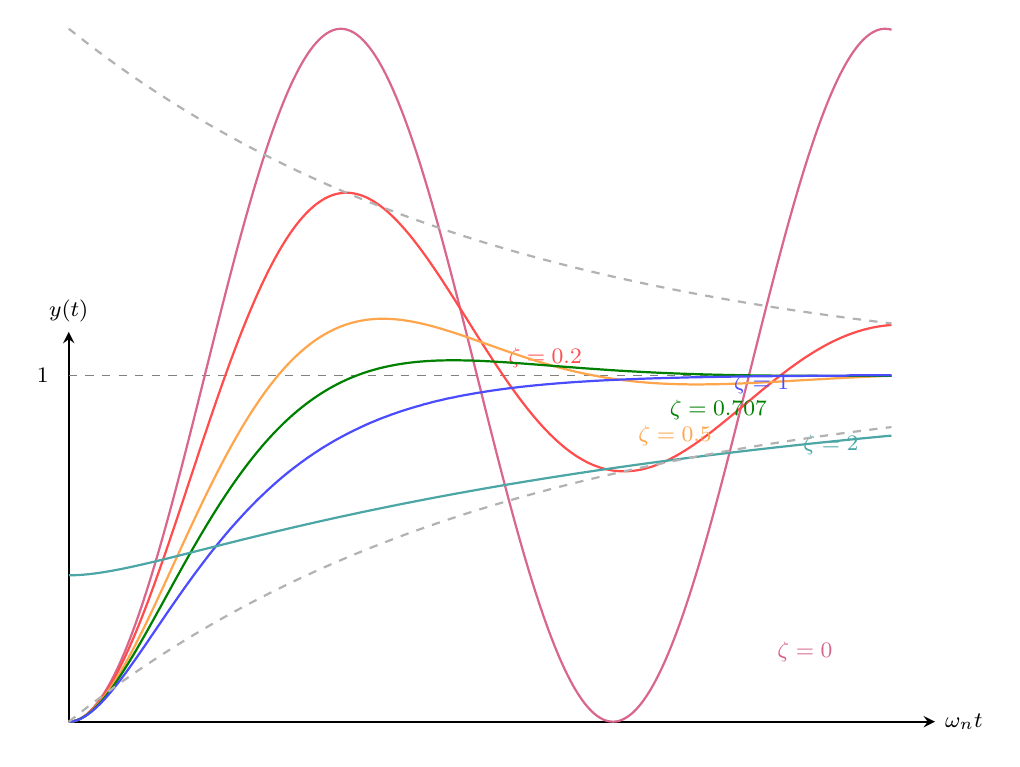
\begin{tikzpicture}[scale=1.1,
    ctrlAx/.style={->,>=stealth,thick},
    ctrlCurve/.style={thick,smooth},
]
\draw[ctrlAx] (0,0) -- (10,0) node[right,font=\footnotesize] {$\omega_n t$};
\draw[ctrlAx] (0,0) -- (0,4.5) node[above,font=\footnotesize] {$y(t)$};
\draw[dashed, gray, thin] (0,4.0) -- (9.5,4.0);
\node[font=\footnotesize] at (-0.3,4.0) {$1$};
% zeta = 0
\draw[ctrlCurve, purple!60, domain=0:9.5, samples=300] plot(\x, {4.0*(1-cos(deg(\x)))});
\node[purple!60, font=\footnotesize] at (8.5,0.8) {$\zeta=0$};
% zeta = 0.2
\draw[ctrlCurve, red!70, domain=0:9.5, samples=300] 
    plot(\x, {4.0*(1 - exp(-0.2*\x)*cos(deg(0.98*\x)) - 0.204*exp(-0.2*\x)*sin(deg(0.98*\x)))});
\node[red!70, font=\footnotesize] at (5.5,4.2) {$\zeta=0.2$};
% zeta = 0.5
\draw[ctrlCurve, orange!70, domain=0:9.5, samples=300] 
    plot(\x, {4.0*(1 - exp(-0.5*\x)*cos(deg(0.866*\x)) - 0.577*exp(-0.5*\x)*sin(deg(0.866*\x)))});
\node[orange!70, font=\footnotesize] at (7.0,3.3) {$\zeta=0.5$};
% zeta = 0.707
\draw[ctrlCurve, green!50!black, domain=0:9.5, samples=300] 
    plot(\x, {4.0*(1 - exp(-0.707*\x)*cos(deg(0.707*\x)) - 1.0*exp(-0.707*\x)*sin(deg(0.707*\x)))});
\node[green!50!black, font=\footnotesize] at (7.5,3.6) {$\zeta=0.707$};
% zeta = 1.0
\draw[ctrlCurve, blue!70, domain=0:9.5, samples=200] 
    plot(\x, {4.0*(1 - (1+\x)*exp(-\x))});
\node[blue!70, font=\footnotesize] at (8.0,3.9) {$\zeta=1$};
% zeta = 2.0
\draw[ctrlCurve, teal!70, domain=0:9.5, samples=200] 
    plot(\x, {4.0*(1 - (2.155/(2*1.732))*exp(-(2-1.732)*0.5*\x) + (0.155/(2*1.732))*exp(-(2+1.732)*0.5*\x))});
\node[teal!70, font=\footnotesize] at (8.8,3.2) {$\zeta=2$};
% Envelope for zeta=0.2
\draw[ctrlCurve, dashed, gray!60, domain=0:9.5, samples=200] plot(\x, {4.0*(1+exp(-0.2*\x))});
\draw[ctrlCurve, dashed, gray!60, domain=0:9.5, samples=200] plot(\x, {4.0*(1-exp(-0.2*\x))});
\end{tikzpicture}
\caption{不同阻尼比$\zeta$下标准二阶系统的单位阶跃响应（$\omega_n$归一化）}
\label{fig:second-order-responses}
\end{figure}

\subsection{临界阻尼与过阻尼响应}

\textbf{临界阻尼}（$\zeta = 1$）：$s_1 = s_2 = -\omega_n$。
\[
Y(s) = \frac{\omega_n^2}{(s+\omega_n)^2} \cdot \frac{1}{s} = \frac{1}{s} - \frac{1}{s+\omega_n} - \frac{\omega_n}{(s+\omega_n)^2}
\]
\[
y(t) = 1 - e^{-\omega_n t}(1 + \omega_n t), \quad t \geq 0
\]

\textbf{过阻尼}（$\zeta > 1$）：两个相异负实极点$s_1 = -(\zeta - \sqrt{\zeta^2-1})\omega_n$，$s_2 = -(\zeta + \sqrt{\zeta^2-1})\omega_n$。
\[
y(t) = 1 - \frac{1}{2\sqrt{\zeta^2-1}}\left( \frac{e^{s_1 t}}{\zeta - \sqrt{\zeta^2-1}} - \frac{e^{s_2 t}}{\zeta + \sqrt{\zeta^2-1}} \right)
\]
过阻尼响应无振荡、无超调，但响应速度随$\zeta$增大而变慢。

\begin{remark}
对实际控制系统，$\zeta$的选择需要在响应速度和超调量之间折中。工程中常取$\zeta \approx 0.707$（即"最佳阻尼比"），此时超调量约$4.3\%$，调节时间最短。随动系统通常选$\zeta = 0.5\sim 0.8$。
\end{remark}

\section{时域性能指标}

时域性能指标基于单位阶跃响应定义，描述系统的暂态品质和稳态精度。

\begin{figure}[H]
\centering
\begin{tikzpicture}[scale=1.1,
    ctrlAxP/.style={->,>=stealth,thick},
    ctrlCurveP/.style={thick,red!70,smooth},
]
\draw[ctrlAxP] (0,0) -- (10,0) node[right,font=\footnotesize] {$t$};
\draw[ctrlAxP] (0,0) -- (0,4.5) node[above,font=\footnotesize] {$y(t)$};
\draw[dashed, gray, thin] (0,3.6) -- (9.5,3.6) node[right,font=\footnotesize] {稳态值};
\draw[dashed, gray, thin] (0,3.78) -- (9.5,3.78);
\draw[dashed, gray, thin] (0,3.42) -- (9.5,3.42);
\node[font=\footnotesize] at (-0.4,3.78) {$1.05$};
\node[font=\footnotesize] at (-0.4,3.42) {$0.95$};
\node[font=\footnotesize] at (-0.4,1.8) {$0.5$};
\node[font=\footnotesize] at (-0.4,0.9) {$0.1$};
\draw[dashed, gray, thin] (0,1.8) -- (0.5,1.8);
\draw[dashed, gray, thin] (0,0.9) -- (0.5,0.9);
% Response curve (simplified)
\draw[ctrlCurveP, domain=0:9.5, samples=300] plot(\x, {3.6*(1 - exp(-0.7*\x)*cos(deg(1.5*\x)) - 0.467*exp(-0.7*\x)*sin(deg(1.5*\x)))});
% Annotations
\draw[<->, blue!60, thick] (1.3, 0.9) -- (1.3, 3.24) node[midway,right,font=\footnotesize,blue!60] {$t_r$};
\draw[dashed, blue!60] (1.3,0.9) -- (1.3,0);
\draw[dashed, blue!60] (1.3,3.24) -- (1.3,3.6);
\draw[<->, green!50!black, thick] (2.3, 3.6) -- (2.3, 4.3) node[midway,right,font=\footnotesize] {$\sigma\%$};
\draw[dashed, green!50!black] (2.3,3.6) -- (9,3.6);
\draw[<->, orange!80, thick] (2.3, 3.8) -- (2.3,3.65);
\draw[dashed, blue!60] (2.3,4.3) -- (2.3,3.8);
\node[font=\footnotesize] at (2.3, -0.4) {$t_p$};
\draw[dashed, blue!60] (2.3, 0) -- (2.3, 4.3);
% t_s region
\draw[<->, purple!70, thick] (0, -0.6) -- (6.5, -0.6) node[midway,below,font=\footnotesize,purple!70] {$t_s$};
\draw[dashed, purple!70] (6.5, 0) -- (6.5, 3.42);
\end{tikzpicture}
\caption{阶跃响应时域性能指标示意}
\label{fig:performance-specs}
\end{figure}

\subsection{上升时间 $t_r$}

响应从稳态值的10\%（或0\%）上升至90\%（或100\%）所需时间。对于欠阻尼二阶系统：
\[
t_r \approx \frac{1 + 0.7\zeta}{\omega_n}
\]

\subsection{峰值时间 $t_p$}

响应达到第一个峰值所需时间。令$\frac{dy}{dt}=0$得：
\[
t_p = \frac{\pi}{\omega_d} = \frac{\pi}{\omega_n\sqrt{1-\zeta^2}}
\]

\subsection{超调量 $\sigma\%$}

定义为超出稳态值的最大幅值与稳态值之比（百分比）：
\[
\sigma\% = \frac{y_{\max} - y(\infty)}{y(\infty)} \times 100\%
\]
将$t_p$代入响应表达式：
\[
\sigma\% = e^{-\pi\zeta/\sqrt{1-\zeta^2}} \times 100\%
\]
超调量仅取决于阻尼比$\zeta$。例如$\zeta=0.5$时$\sigma\% \approx 16.3\%$，$\zeta=0.707$时$\sigma\% \approx 4.3\%$，$\zeta=1$时$\sigma\%=0$。

\subsection{调节时间 $t_s$}

响应进入并保持在稳态值$\pm\Delta$（通常$\Delta=2\%$或$5\%$）误差带内所需的最短时间。
对于欠阻尼系统，由衰减包络$1\pm e^{-\zeta\omega_n t_s}/\sqrt{1-\zeta^2} = 1\pm\Delta$，取$\Delta=2\%$：
\[
t_s \approx \frac{4}{\zeta\omega_n} \quad (2\%\text{准则}), \qquad
t_s \approx \frac{3}{\zeta\omega_n} \quad (5\%\text{准则})
\]

\begin{remark}
四个性能指标之间相互制约。增大$\omega_n$可同时减小$t_r$和$t_p$，但不影响$\sigma\%$。增大$\zeta$可减小$\sigma\%$和振荡次数，但会增大$t_r$。设计者必须在这些指标之间进行合理的折中。
\end{remark}

\subsection*{Python示例：二阶系统时域性能指标计算}

\begin{lstlisting}[language=Python]
import numpy as np
from scipy import signal

def second_order_performance(zeta, wn, delta=0.02):
    """计算二阶系统的时域性能指标"""
    wd = wn * np.sqrt(1 - zeta**2)
    sigma = np.exp(-np.pi * zeta / np.sqrt(1 - zeta**2))

    tr = (1 + 0.7*zeta) / wn           # 近似上升时间
    tp = np.pi / wd                     # 峰值时间
    ts = 4.0 / (zeta * wn) if delta == 0.02 else 3.0 / (zeta * wn) # 调节时间

    print(f"阻尼比 zeta = {zeta:.3f}")
    print(f"自然频率 omega_n = {wn:.2f} rad/s")
    print(f"上升时间 t_r = {tr:.3f} s")
    print(f"峰值时间 t_p = {tp:.3f} s")
    print(f"超调量 sigma = {sigma*100:.2f}%")
    print(f"调节时间 t_s ({delta*100:.0f}%) = {ts:.3f} s")

    # 仿真验证
    num = [wn**2]
    den = [1, 2*zeta*wn, wn**2]
    sys = signal.TransferFunction(num, den)
    t, y = signal.step(sys)
    y_max_idx = np.argmax(y)
    print(f"仿真超调量 = {(y[y_max_idx]-1.0)*100:.2f}%")
    print(f"仿真峰值时间 = {t[y_max_idx]:.3f} s")
    print("-" * 40)

# 示例
second_order_performance(0.4, 2.0)
second_order_performance(0.707, 2.0)
second_order_performance(0.9, 2.0)
\end{lstlisting}

\section{稳态误差分析}

\subsection{终值定理与稳态误差}

稳态误差定义为$e_{ss} = \lim_{t\to\infty} e(t) = \lim_{t\to\infty}[r(t)-y(t)]$。当$e(t)$的Laplace变换$E(s)$满足终值定理条件时：
\[
e_{ss} = \lim_{t\to\infty} e(t) = \lim_{s\to 0} sE(s)
\]

对于单位反馈系统（$H(s)=1$），误差传递函数为$\Phi_e(s) = 1/(1+G(s))$，故：
\[
e_{ss} = \lim_{s\to 0} s \cdot \frac{1}{1+G(s)} \cdot R(s)
\]

\subsection{系统型别与静态误差系数}

设开环传递函数$G(s)$的标准形式为：
\[
G(s) = \frac{K (\tau_1 s+1)(\tau_2 s+1)\cdots(\tau_q s+1)}{s^N (T_1 s+1)(T_2 s+1)\cdots(T_p s+1)}
\]
其中$N$为积分环节个数（$s=0$处极点的重数），称为系统\textbf{型别}。

定义三个静态误差系数：
\begin{itemize}
\item 位置误差系数：$K_p = \lim_{s\to 0} G(s)$
\item 速度误差系数：$K_v = \lim_{s\to 0} sG(s)$
\item 加速度误差系数：$K_a = \lim_{s\to 0} s^2 G(s)$
\end{itemize}

\begin{myformula}
\textbf{不同型别系统在不同输入下的稳态误差：}
\text{阶跃输入} (R(s)=1/s):\quad e_{ss} &= \frac{1}{1+K_p} \\
\text{斜坡输入} (R(s)=1/s^2):\quad e_{ss} &= \frac{1}{K_v} \\
\text{抛物线输入} (R(s)=1/s^3):\quad e_{ss} &= \frac{1}{K_a}
\end{myformula}

\begin{table}[H]
\centering
\caption{系统型别与稳态误差}
\label{tab:steady-state-error}
\renewcommand{\arraystretch}{1.5}
\begin{tabular}{|c|c|c|c|c|c|c|c|}
\hline
\textbf{型别} & $K_p$ & $K_v$ & $K_a$ & $e_{ss}$(阶跃) & $e_{ss}$(斜坡) & $e_{ss}$(抛物线) \\ \hline
0型 & $K$ & 0 & 0 & $1/(1+K)$ & $\infty$ & $\infty$ \\ \hline
I型 & $\infty$ & $K$ & 0 & 0 & $1/K$ & $\infty$ \\ \hline
II型 & $\infty$ & $\infty$ & $K$ & 0 & 0 & $1/K$ \\ \hline
\end{tabular}
\end{table}

从表中可见，提高系统型别可以消除对低阶输入的稳态误差，但型别越高，稳定性设计越困难——这反映了控制理论中"精度"与"稳定性"之间的本质矛盾。

\begin{figure}[H]
\centering
\begin{tikzpicture}[scale=1.0,
    ctrlAxS/.style={->,>=stealth,thick},
    ctrlCurveS/.style={thick,smooth},
]
% Steady-state error demo for step input - type 0 vs type 1
\begin{scope}[xshift=-4cm, yshift=0cm]
\draw[ctrlAxS] (0,0) -- (5,0) node[right,font=\footnotesize] {$t$};
\draw[ctrlAxS] (0,0) -- (0,3.5) node[above,font=\footnotesize] {$y(t)$};
\draw[dashed, gray] (0,2.5) -- (5,2.5) node[right,font=\footnotesize] {$r(t)=1$};
% Type 0
\draw[ctrlCurveS, blue!60] plot[domain=0:4.8, samples=100] (\x, {2.5*0.8*(1-exp(-1.0*\x))});
\node[blue!60, font=\footnotesize] at (3.5,1.6) {0型: $e_{ss}\neq 0$};
\draw[<->, red] (4.0, 2.5) -- (4.0, 2.0);
\node[red, font=\footnotesize] at (4.0, 2.25) [right] {$e_{ss}$};
% Type I
\draw[ctrlCurveS, green!50!black] plot[domain=0:4.8, samples=100] (\x, {2.5*(1-exp(-1.5*\x))});
\node[green!50!black, font=\footnotesize] at (2.0,2.9) {I型以上: $e_{ss}=0$};
\end{scope}
% Steady-state error for ramp input - type 0 vs type I
\begin{scope}[xshift=4cm, yshift=0cm]
\draw[ctrlAxS] (0,0) -- (5,0) node[right,font=\footnotesize] {$t$};
\draw[ctrlAxS] (0,0) -- (0,3.5);
\draw[ctrlCurveS, gray, dashed] (0,0) -- (4.5,3.0) node[right,font=\footnotesize] {$r(t)=t$};
% Type I
\draw[ctrlCurveS, blue!60] plot[domain=0:4.5, samples=100] (\x, {\x - 0.5*(1-exp(-2.0*\x))});
\node[blue!60, font=\footnotesize] at (3.0,2.2) {I型: $e_{ss}=1/K_v$};
% Type 0
\draw[ctrlCurveS, red!70] plot[domain=0:4.5, samples=100] (\x, {0.6*(1-exp(-1.0*\x))});
\node[red!70, font=\footnotesize] at (4.0,0.4) {0型: 不能跟踪};
\end{scope}
\end{tikzpicture}
\caption{不同型别系统的稳态误差示意（左：阶跃响应；右：斜坡响应）}
\label{fig:steady-state-demo}
\end{figure}

\section{稳定性代数判据}

\subsection{稳定性概念与充要条件}

\begin{mydefinition}{BIBO稳定性}
线性时不变系统是BIBO（有界输入-有界输出）稳定的，当且仅当系统的所有闭环极点均位于$s$平面的左半平面（即具有负实部）。
\end{mydefinition}

\begin{myTheorem}{稳定性充要条件}
连续时间LTI系统稳定的充要条件是其闭环特征方程
\[
\Delta(s) = a_n s^n + a_{n-1}s^{n-1} + \cdots + a_1 s + a_0 = 0
\]
的所有根均具有负实部（即位于左半$s$平面）。
\end{myTheorem}

直接求解高阶特征方程的根是困难的。Routh和Hurwitz分别于1877年和1895年提出了仅需代数运算即可判断稳定性的方法——无需实际求解特征根。

\subsection{Routh-Hurwitz判据}

\begin{myTheorem}{Routh-Hurwitz稳定性判据}
特征多项式$\Delta(s) = a_n s^n + a_{n-1}s^{n-1} + \cdots + a_0$（$a_n > 0$）的所有根均具有负实部的必要条件是：
\begin{enumerate}
\item 特征多项式各项系数均存在且同号（即$a_i > 0$，对所有$i = 0,1,\dots,n$）。
\end{enumerate}
充分条件（Routh判据）：构造Routh表，若Routh表第一列所有元素均大于零，则系统稳定。若第一列元素符号改变$m$次，则特征方程有$m$个根位于右半平面。
\end{myTheorem}

\subsection{Routh表的构造}

对于特征多项式$\Delta(s) = a_n s^n + a_{n-1}s^{n-1} + a_{n-2}s^{n-2} + \cdots + a_1 s + a_0$，构造Routh表如下：

\begin{figure}[H]
\centering
\begin{tikzpicture}[
    ctrlRow/.style={font=\footnotesize},
]
% Routh table
\node[ctrlRow] at (0,3.5) {$s^n$：};
\node[ctrlRow] at (2.5,3.5) {$a_n$};
\node[ctrlRow] at (4.5,3.5) {$a_{n-2}$};
\node[ctrlRow] at (6.5,3.5) {$a_{n-4}$};
\node[ctrlRow] at (8.5,3.5) {$\cdots$};

\node[ctrlRow] at (0,2.5) {$s^{n-1}$：};
\node[ctrlRow] at (2.5,2.5) {$a_{n-1}$};
\node[ctrlRow] at (4.5,2.5) {$a_{n-3}$};
\node[ctrlRow] at (6.5,2.5) {$a_{n-5}$};
\node[ctrlRow] at (8.5,2.5) {$\cdots$};

\node[ctrlRow] at (0,1.5) {$s^{n-2}$：};
\node[ctrlRow] at (2.5,1.5) {$b_1$};
\node[ctrlRow] at (4.5,1.5) {$b_2$};
\node[ctrlRow] at (6.5,1.5) {$b_3$};
\node[ctrlRow] at (8.5,1.5) {$\cdots$};

\node[ctrlRow] at (0,0.5) {$s^{n-3}$：};
\node[ctrlRow] at (2.5,0.5) {$c_1$};
\node[ctrlRow] at (4.5,0.5) {$c_2$};
\node[ctrlRow] at (6.5,0.5) {$c_3$};
\node[ctrlRow] at (8.5,0.5) {$\cdots$};

\node[ctrlRow] at (0,-0.5) {$\ \vdots$};
\node[ctrlRow] at (0,-1.3) {$s^0$：};
\node[ctrlRow] at (2.5,-1.3) {$p_1$};

% Formula annotations
\node[ctrlRow, align=left] at (5.0, -2.5) {
$b_1 = \frac{a_{n-1}a_{n-2} - a_n a_{n-3}}{a_{n-1}}$，\quad
$b_2 = \frac{a_{n-1}a_{n-4} - a_n a_{n-5}}{a_{n-1}}$，\quad
$\cdots$\\
$c_1 = \frac{b_1 a_{n-3} - a_{n-1} b_2}{b_1}$，\quad
$c_2 = \frac{b_1 a_{n-5} - a_{n-1} b_3}{b_1}$，\quad
$\cdots$
};
\end{tikzpicture}
\caption{Routh表的构造规则示意}
\label{fig:routh-table}
\end{figure}

表的构造规则：第$k$行的元素利用第$(k-1)$行和第$(k-2)$行的前两列元素按"十字交叉"法则计算：
\[
\text{新元素} = \frac{(\text{上一行第一列})\times(\text{上二行下一列}) - (\text{上二行第一列})\times(\text{上一行下一列})}{\text{上一行第一列}}
\]

\subsection{Routh判据的特殊情况}

\textbf{情况一：Routh表某行第一列元素为零，该行其余元素不全为零。}

处理方法：用一个小的正数$\varepsilon$代替零，继续计算Routh表，然后令$\varepsilon \to 0^+$检查第一列符号变化。

\textbf{情况二：Routh表某行整行全为零。}

这表明特征方程存在大小相等、符号相反的根（即关于原点对称的根对），如$\pm\sigma$、$\pm j\omega$或$\pm\sigma\pm j\omega$。处理方法：
\begin{enumerate}
\item 利用上一行（全零行的上一行）的元素构造辅助多项式$A(s)$。
\item 对$A(s)$求导得$dA(s)/ds$，用其系数代替全零行。
\item 辅助方程$A(s)=0$的根即为对称根，可通过求解$A(s)=0$获得。
\end{enumerate}

\begin{example}
判断特征方程$\Delta(s) = s^4 + s^3 + 3s^2 + 2s + 2 = 0$对应系统的稳定性。

构造Routh表：
\[
\begin{array}{c|ccc}
s^4: & 1 & 3 & 2 \\
s^3: & 1 & 2 & 0 \\
s^2: & \frac{1\cdot 3 - 1\cdot 2}{1}=1 & \frac{1\cdot 2 - 1\cdot 0}{1}=2 & \\
s^1: & \frac{1\cdot 2 - 1\cdot 2}{1}=0 & \cdots & \\
\end{array}
\]

$s^1$行第一列为零！用$\varepsilon$代替：$s^1$行为$\varepsilon$、$0$；$s^0$行为$\frac{\varepsilon\cdot 0 - 1\cdot 0}{\varepsilon}=0$（或直接计算为$2$）。仔细计算：$s^1$行元素为$(\varepsilon \cdot 2 - 1\cdot 0)/\varepsilon = 2$。第一列：$1,1,1,\varepsilon,2$。当$\varepsilon \to 0^+$时符号不变，但需要进一步检查$s^1$行对应的辅助项。

实际上计算后得辅助多项式$A(s)=s^2+2$，求导得$2s$，$s^1$行系数为$[2,0]$，$s^0$行为$2$。第一列全为正——系统稳定。但辅助方程$s^2+2=0$给出$s=\pm j\sqrt{2}$，表明系统有一对纯虚极点——临界稳定。
\end{example}

\subsection*{Python示例：Routh判据实现}

\begin{lstlisting}[language=Python]
import numpy as np

def routh_table(coeffs):
    """构造Routh表，输入特征多项式系数（降幂）"""
    n = len(coeffs) - 1  # 阶次
    rows = n + 1
    cols = (n + 2) // 2
    table = np.zeros((rows, cols))

    # 填充前两行
    for j in range(cols):
        if 2*j < len(coeffs):
            table[0, j] = coeffs[2*j]
        if 2*j + 1 < len(coeffs):
            table[1, j] = coeffs[2*j + 1]

    # 计算后续行
    for i in range(2, rows):
        for j in range(cols - 1):
            if abs(table[i-1, 0]) < 1e-12:
                # 首列为零，用eps替代
                table[i-1, 0] = 1e-6
            table[i, j] = (table[i-1, 0] * table[i-2, j+1] - 
                           table[i-2, 0] * table[i-1, j+1]) / table[i-1, 0]

    print("Routh表第一列:", table[:, 0])
    sign_changes = sum(1 for i in range(1, len(table[:, 0]))
                       if table[i-1, 0] * table[i, 0] < 0)
    if sign_changes > 0:
        print(f"不稳定！右半平面极点个数 = {sign_changes}")
    else:
        print("所有极点均位于左半平面（或虚轴），系统稳定。")
    return table

# 测试：s^4 + 2s^3 + 3s^2 + 4s + 5
coeffs = [1, 2, 3, 4, 5]
routh_table(coeffs)

# 测试：s^3 + s^2 + 2s + 24
coeffs2 = [1, 1, 2, 24]
routh_table(coeffs2)
\end{lstlisting}

\begin{remark}
Routh-Hurwitz判据是经典控制理论中最优雅的成果之一——它仅需乘除运算即可判定特征方程的稳定性，无需进行多项式求根。然而它只能回答"是否稳定"，无法给出稳定程度（相对稳定性）。对于相对稳定性的评估，将在第四章（根轨迹法）和频域分析中进一步讨论。
\end{remark}

\section*{本章小结}

本章从时域角度全面分析了控制系统的动态与稳态行为。一阶和二阶系统是理解高阶系统响应的基础——高阶系统的主极点可以通过降阶近似为低阶标准型进行分析。时域性能指标（$t_r, t_p, \sigma\%, t_s$）是刻画暂态品质的定量标准，其解析表达式揭示了系统参数（$\zeta$和$\omega_n$）与性能之间的函数关系。稳态误差分析则通过终值定理和静态误差系数建立系统型别与跟踪精度的联系。Routh-Hurwitz判据作为稳定性代数判据，是系统综合设计中的第一道检验。
